\documentclass[a4paper,french,bookmarks]{article}
\usepackage{./Structure/4PE18TEXTB}

\begin{document}
\stylizeDoc{Mathématiques}{Chapitre 14}{Matrices}

\initcours{}

\section{Présentation}

\subsection{Définitions}

\begin{definition}{Matrice}{}
    Soient $(n, p) \in {\bdN^*}^2$. Une \bf{matrice de type $(n, p)$} à coefficients dans $\bdK$ est une famille $(a_{i, j})_{\substack{1 \leq i \leq n\\1 \leq j \leq p}}$ d'éléments de $\bdK$.
\end{definition}
On pourrait écrire de manière équivalente cette famille $A = (a_{i,j})_{(i, j) \in \llbracket 1, n\rrbracket \times \llbracket 1, p\rrbracket}$. Pour travailler de manière aisée avec les matrices, on utilisera pour ces dernières une représentation planaire. Pour la matrice $A$, on aurait :

\[ A = \begin{pmatrix}
a_{1,1} & a_{1,2} & \dots & a_{1,i} & \dots & a_{1,p}\\
a_{2,1} & a_{2,2} & \dots & a_{2, i} & \dots & a_{2,p}\\
\vdots & & \ddots& & & \vdots\\
a_{j, i} & a_{j, i} & \dots & a_{j, i} & \dots &a_{j, p}\\
\vdots & & & & \ddots & \vdots\\
a_{n, 1} & a_{n, 2} & \dots & a_{i, n} &\dots &a_{n, p}
\end{pmatrix}\]

On remarquera que $A$ possède $n \times p$ coefficient, et que le coefficient $a_{i, j}$ est coefficient de ligne $i$ et de colonne $j$. A ce titre, le premier indice $(i)$ désigne donc la ligne et le second indice $(j)$ désigne la colonne. La matrice $A$ a donc $p$ colonnes et $n$ lignes. Le coefficient $a_{i, j}$ de la matrice $A$ sera aussi noté $a_{ij}$, $[A]_{i, j}$ ou $[A]_{ij}$.

\begin{definition}{Ensemble des matrices de type $(n, p)$}{}
    Soient $(n, p) \in {\bdN^*}^2$. \bf{L'ensemble des matrices de type $(n, p)$} à coefficient dans $\bdK$ est noté \hg{$\bcM_{n, p}(\bdK)$}.
\end{definition}

On peut alors définir la notion d'égalité de deux matrices, dans la mesure où elles sont de même \guill{type}.

\begin{definition}{Égalité dans $\bcM_{n, p}(\bdK)$}{}
     Soient $(n, p) \in {\bdN^*}^2$. Soient $A=(a_{i, j})_{(i, j) \in \llbracket 1, n\rrbracket \times \llbracket 1, p\rrbracket} \in \bcM_{n, p}(\bdK)$ et $B=(b_{i, j})_{(i, j) \in \llbracket 1, n\rrbracket \times \llbracket 1, p\rrbracket} \in \bcM_{n, p}(\bdK)$.
    
    \[ \hg{A = B \iff \forall (i, j) \in \llbracket 1, n\rrbracket \times \llbracket 1, p\rrbracket}, \quad a_{i, j} = b_{i, j}\]
\end{definition}

\begin{example}{}{}
    \begin{enumerate}
        \ithand $A = \left((-1)^{i+j}\right) \in \bcM_{2, 4}(\bdR)$. On a alors :
        
        \[ \hg{A = \begin{pmatrix}
            1 & -1 & 1 & -1\\
            -1 & 1 & -1 & 1
        \end{pmatrix}}\]
        
        \ithand $B = \left(\min{i, j}\right) \in \bcM_{n, n}(\bdR)$
        
        \[ \hg{B = \begin{pmatrix}
            1 & 1 & 1 & \dots & 1\\
            1 & 2 & 2 & \dots & 2\\
            1 & 2 & 3 & \dots & 3\\
            \vdots & & & \ddots & \vdots\\
            1 & 2 & 3 &\dots & n
        \end{pmatrix}}\]
    \end{enumerate}
\end{example}

\subsection{Lignes et colonnes}

\begin{definition}{Matrice-ligne}{}
     Soit $n \in \bdN^*$. Une \bf{matrice-ligne} est une matrice \hg{$A \in \bcM_{1, n}(\bdK)$}
     
     \[ \hg{A = \begin{pmatrix}a_{1, 1}& a_{2, 1} & \dots & a_{n, 1}
     \end{pmatrix}}\]
\end{definition}

\begin{definition}{Matrice-colonne}{}
     Soit $n \in \bdN^*$. Une \bf{matrice-colonne} est une matrice \hg{$A \in \bcM_{n, 1}(\bdK)$}.
     
     \[ \hg{A = \begin{pmatrix}a_{1, 1}\\
     a_{2, 1}\\
     \vdots\\
     a_{n, 1}
     \end{pmatrix}}\]
\end{definition}

\subsection{Matrices carrées}

On s'intéresse au cas où $n = p$. On étudie alors les \guill{matrices carrées}.

\begin{definition}{Matrice carrées}{}
     Soit $n \in \bdN^*$.  Une \bf{matrice-colonne} est une matrice \hg{$A \in \bcM_{n, n}(\bdK)$}.
\end{definition}

On peut donc également simplifier la notation de l'ensemble des matrices carrées.

\begin{definition}{$\bcM_n(\bdK)$}{}
    Soit $n \in \bdN^*$. On note \bf{$\bcM_n(\bdK)$ l'ensemble des matrices carrées} de taille $n \times n$.
     \[ \hg{\bcM_n(\bdK) = \bcM_{n, n}(\bdK)}\]
\end{definition}

\begin{definition}{coefficients diagonaux}{}
    Soit $n \in \bdN^*$, $A \in \bcM_n{\bdK}$ et $(i, j) \in \llbracket 1, n\rrbracket^2$. On dit que \bf{le coefficient $[A]_{i, j}$ est diagonal} si et seulement si $i = j$.
\end{definition}

Les coefficients diagonaux sont donc les coefficients situés sur la \guill{diagonale} partant d'en haut à gauche, à en bas à droite de la matrice :

\[ A = \begin{pmatrix}
    a_{1, 1} \\
    & a_{2, 2}\\
    & & \ddots\\
    & & & a_{n, n}
    \end{pmatrix} \]

On remarquera que, dans le cas particulier où $n = 1$, on pourra identifier $\bcM_1(\bdK)$ à $\bdK$.

\begin{definition}{Matrice diagonale}{}
    Soit $n \in \bdN^*$, $A \in \bcM_n(\bdK)$. On dit que \bf{$A$ est diagonale} si et seulement si :
    
    \[ \hg{\forall (i, j) \in \llbracket 1, n\rrbracket^2, \qquad i \neq j \implies [A]_{i, j} = 0}\]
\end{definition}

Si $A$ est diagonale, on écrira $A = \diag(a_{1, 1}, a_{2, 2}, \dots, a_{n, n})$

\begin{definition}{Ensemble des matrices diagonales}{}
    Soit $n \in \bdN^*$. \bf{L'ensemble des matrices diagonales} de $\bcM_n(\bdK)$ est noté \hg{$\bcD_n(\bdK)$}.
\end{definition}

\begin{example}{}{}
    \begin{enumerate}
        \ithand 
        
        \ithand Soit $\lambda \in \bdK$. La matrice d'homothétie de facteur $\lambda$ est diagonale :
        
        \[\diag(\lambda, \lambda, \dots, \lambda) = \begin{pmatrix}
            \lambda & & (O) \\
            & \ddots & \\
            (0) & & \lambda
        \end{pmatrix}
        \]
    \end{enumerate}
\end{example}

Matrices triangulaires

\subsection{Groupe $(M_{n, p}(\bdK), +)$}

\subsection{Produit matriciel}

\begin{definition}{Produit scalaire}{}
    Soit $n, \in \bdN^*$, $L=\begin{pmatrix}a_1 & a_2 & \ldots & a_n\end{pmatrix}
    \in \bcM_{1, n}(\bdK)$ et $C = \begin{pmatrix}b_1 \\ a_2 \\ \vdots \\ a_n\end{pmatrix} \in \bcM_{n, 1}(\bdK)$. 
    
    Le \bf{produit $L\times C$} est défini par le scalaire $\displaystyle \sum_{k=1}^n a_{1, k}b_{k, 1} \in \bdK$. Précisément :
    
    \[ \hg{\times : \begin{array}[t]{ccc}
        \bcM_{1, n}(\bdK)\times\bcM_{n, 1}(\bdK) &\to& \bdK  \\
        \left((a_{i, j})_{(i, j) \in \{1\}\times\llbracket1, n\rrbracket}, (b_{i, j})_{(i, j) \in \llbracket1, n\rrbracket\times\{1\}}\right) &\mapsto& \displaystyle \sum_{k=1}^n a_{1, k}b_{k, 1}
    \end{array}}\]
\end{definition}

On peut alors généraliser ce produit à une matrice $A \in \bcM_{n, p}(\bdK)$ et $B \in \bcM_{p, q}(\bdK)$.

\begin{theorem}{Produit de matrices élémentaires}{}
    \[ \hg{E_{i_0, j_0} \times E_{k_0, l_0} = \delta_{j_0, k_0}E_{i_0, l_0}}\]
\end{theorem}

\demoth{
    Notons $C = E_{i_0, j_0} \times E_{k_0, l_0}$.
    
    \begin{enumerate}
        \ithand Si $i \neq i_0$, $C_{i, j} = 0$ car la ligne $i$ de $E_{i_0, j_0}$ est nulle.
        
        \ithand Si $j \neq l_0$, $C_{i, j} = 0$ car la colonne $i$ de $E_{k_0, l_0}$ est nulle.
        
        \ithand Il reste donc :
        
        \[ [C]_{i_0, l_0} =  \sum_{k} [E_{i_0, j_0}]_{i_0, k}\times[E_{k_0, l_0}]_{k, l_0} = \sum_{k} \delta_{j_0, k}\times\delta{k_0, k}=\left\lbrace\begin{array}{ll}
            1 &\text{si} \ j_0 = k_0  \\
            0 &\text{sinon} 
        \end{array}\right.\]
    \end{enumerate}
}

\subsection{Propriétés du produit matriciel}

Sous réserve de dimensions compatibles :

\begin{property}{Associativité}{}
    \[ \hg{(AB)C = A(BC)}\]
\end{property}

\demo{
    On montre pour tout $i$ et tout $j$, on a $[(AB)C]_{i, j} = [A(BC)]_{i, j}$.
}

\begin{property}{Neutres à gauche et à droite}{}
    Soient $n, p \in {\bdN^*}^2$ et $A \in \bcM_{n, p}(\bdK)$. On a :
    
    \[ \hg{I_n\times A = A \times I_p = A}\]
\end{property}

\begin{property}{Distributivité}{}
    
    
    \[ \hg{A\times(B + C) = A\times B + A \times C \qquad\et\qquad (A + B)\times C = AC + BC}\]
\end{property}

\subsection{Matrices inversibles}
    
\begin{definition}{Matrice inversible}{}
    Soit $A \in \bcM_n(\bdK)$ une matrice carrée. $A$ est \bf{inversible} si et seulement si
    
    \[ \hg{\exists B \in \bcM_n(\bdK), \qquad AB = BA = I_n}\]
\end{definition}
Alors, $B$ est l'inverse de $A$ et on note $B = A^{-1}$.

\begin{definition}{$GL_n(\bdK)$}{}
    On note \bf{$GL_n(\bdK)$} l'ensemble des \bf{matrices inversibles}.
    
    \[\hg{\bcM_n(\bdK)^* = GL_n(\bdK)}\]
\end{definition}

\begin{property}{Groupe $(GL_n(\bdK), \times)$}{}
    \bf{$(GL_n(\bdK), \times)$} est \bf{un groupe multiplicatif}.
\end{property}

\demo{
    Immédiat par propriétés de cours.
}

\begin{theorem}{}{}
    Soit $A \in \bcM_n(\bdK)$. On a équivalence entre :
    
    \[ A \in GL_n(\bdK) \iff \exists B \in \bcM_n(\bdK), \ AB = I_n \iff \exists C \in \bcM_n(\bdK), \ CA = I_n\]
\end{theorem}

\demoth{
    Admis provisoirement.
}

\newpage
\begin{example}{}{}
    Soit $A = \begin{pmatrix}0 & 1 & 0\\ -1 & 2 & 0\\ 1 & 0 & -1\end{pmatrix}$.
    
    \begin{enumerate}
        \item Calculer $A^2$ et $A^3$.
        \item Calculer $A^3 - A^2 - A$
        \item Montrer que $A$ est inversible et donner $A^{-1}$
        \item Calculer les puissances $A^n$, $n \in \bdN$.
    \end{enumerate}
    \tcblower
    
    \begin{enumerate}
        \item On obtient \hg{$A^2 = \begin{pmatrix}-1 & 2 & 0\\ -1 & 3 & 0\\ -1 1 1\end{pmatrix}$} et \hg{$A^3 = \begin{pmatrix}-2 & 3 & 0\\ -3 & 4 & 0\\ 0 & 1 & -1\end{pmatrix}$}.
        
        \item On a \hg{$A^3 - A^2 - A = \begin{pmatrix}-1 & 0 & 0\\ 0 & -1 & 0\\ 0 & 0 & -1\end{pmatrix} = -I_3$}.
        
        \item On a $A^3 - A^2 - A = -I_3$ donc $A\times\left[I_3 + A - A^2\right] = I_3$.
        
        Donc $A$ est inversible et $A^{-1} = I_3 + A - A^2$ avec \hg{$A^{-1} \begin{pmatrix}0 & -1 & 0\\ 1 & 0 & 0\\ 0 & -1 & -1\end{pmatrix}$}
        
        \item On va poser $P(X) = X^3 - X^2 - X + 1$. On constate que \bf{$P$ est un polynôme annulateur de $A$} car $P(A) = A^3 - A^2 - A + I = 0_3$.
        
        Soit $n \in \bdN$. Posons la divisions euclidienne de $X^n$ par $P(X)$.
    \end{enumerate}
\end{example}

\begin{theorem}{}{}
    Soit $A = \begin{pmatrix}
                a & b\\
                c & d
            \end{pmatrix} \in \bcM_2(\bdK)$. On a :
            
    \[ \hg{A \in GL_2(\bdK) \iff \det A \neq 0} \]
\end{theorem}

\demoth{
    Soit $A = \begin{pmatrix}
                a & b\\
                c & d
            \end{pmatrix} \in \bcM_2(\bdK)$. On a :
            
    \[ A^2 = \begin{pmatrix}
                a^2+bc & ab+bd\\
                ca+dc & bc+d^2
            \end{pmatrix} = \begin{pmatrix}
                a^2+bc & b(a+d)\\
                c(a+d) & bc+d^2
            \end{pmatrix}\]
            
    Or $(a+d)A = \begin{pmatrix}
                a^2+ad & b(a+d)\\
                c(a+d) & ad+d^2
            \end{pmatrix}$, donc :
            
    \[A^2 - (a+d)A = \begin{pmatrix}
                bc-ad & 0\\
                0 & bc-ad
            \end{pmatrix} = (bc-ad)\begin{pmatrix}
                1 & 0\\
                0 & 1
            \end{pmatrix} = (\det A)I_2\]
    
    \begin{enumerate}
        \ithand Si $\det A = ad-bc \neq 0$, alors :
        
        \[ \dfrac{1}{bc-ad}\left[a^2 - (a+d)A\right] = I_2 \qquad\text{donc}\qquad A \times \left[\dfrac{A-(a+d)I_2}{bc-ad}\right] = I_2\]
        
        On a bien trouvé $B \in \bcM_2(\bdK)$ tel que $AB = I_2$, donc $A \in GL_2(\bdK)$ et :
        
        \[ A^{-1} = \dfrac{A-(a+d)I_2}{bc-ad} = \dfrac{1}{\det A}\left[\begin{pmatrix}
                a+d & 0\\
                0 & a+d
            \end{pmatrix} - \begin{pmatrix}
                a & b\\
                c & d
            \end{pmatrix}\right] = \dfrac{1}{\det A}\begin{pmatrix}
                d & -b\\
                -c & a
            \end{pmatrix}\]
            
            \ithand Si $\det A = ad + bc = 0$, alors :
            
            \[ A^2 - (a+d)A = 0_2 \quad\text{donc}\quad A^2 = (a+d)A \quad\text{donc si $A$ est inversible}\quad A = (a+d)I_2\]
            
            On aurait alors $\begin{pmatrix}
                a & b\\
                c & d
            \end{pmatrix} = \begin{pmatrix}
                a+d & 0\\
                0 & a+d
            \end{pmatrix}$, et donc $b = c = 0$ et $a = a+d$ d'où $d = 0$, et $d = d+a$ d'où $a = 0$.
            
            Donc $A = \begin{pmatrix}
                0 & 0\\
                ° & 0
            \end{pmatrix} = 0_2$ ce qui absurde car $0_2$ n'est pas inversible, donc $A$ n'est pas inversible.
            
            \ithand Par contraposée dans le deuxième cas, on obtient bien en conclusion :
            
            \[ A \in GL_2(\bdK) \iff \det A \neq 0 \]
    \end{enumerate}
}
\newpage

\section*{Méthode du pivot de Gauss-Jordan}

Soit une matrice $A$. La matrice $A$ est-elle inversible ? Et si oui, comment calculer $A^{-1}$ ?

On peut pour cela utilise l'algorithme du pivot de Gauss-Jordan. En partant de $(A \mid I_3)$, et en opérant sur les lignes, on cherchera à arriver progressivement à $(I_3 \mid A^{-1})$.

\begin{example}{}{}
    Prenons comme exemple la matrice $A$ suivante :
    
    \[ \hg{A = \left(\begin{array}{ccc}
        1  & 0 & -1  \\
        2  & 1 & -3  \\
        -1 & 0 & 2
    \end{array}\right)}\]
    
    \tcblower
    
    \begin{align*}
         \left(\begin{array}{ccc|ccc}
        \boxedcol{\hg{1}} & 0 & -1 & 1 & 0 & 0 \\
        2  & 1 & -3 & 0 & 1 & 0 \\
        -1 & 0 & 2 & 0 & 0 & 1
    \end{array}\right) &&\asymp{\substack{L_2 \leftarrow L_2 - 2L_1\\L_3\leftarrow L_3 + L_1}}&& \left(\begin{array}{ccc|ccc}
        1  & 0 & -1 & 1 & 0 & 0 \\
        0  & \boxedcol{\hg{1}} & -1 & -2 & 1 & 0 \\
        0 & 0 & 1 & 1 & 0 & 1
    \end{array}\right)\\
    &&\asymp{\substack{L_2 \leftarrow L_2 + L_3\\L_1\leftarrow L_1 + L_3}}&& \left(\vphantom{\begin{array}{c}
        1 \\ 2 \\ 3
    \end{array}}\right.\hg{\underbrace{\begin{array}{ccc}
        1 & 0 & 0   \\
        0 & 1 & 0 \\
        0 & 0 & 1
    \end{array}}_{I_3}}\left|\vphantom{\begin{array}{c}
        1 \\ 2 \\ 3
    \end{array}}\right.\boxedcol{\underbrace{\begin{array}{ccc}
        2 &0 & 1  \\
        -1 &1 & 1 \\
        1 & 0 & 1
    \end{array}}_{A^{-1}}}\left.\vphantom{\begin{array}{c}
        1 \\ 2 \\ 3
    \end{array}}\right)
    \end{align*}
    
    On arrive bien à obtenir la matrice identité $I_3$ à gauche, et on obtient ainsi la matrice $A^{-1}$ à droite :
    
    \[ \hg{A^{-1} = \begin{pmatrix}
        2 & 0 & 1\\
        -1 & 1 & 1\\
        1 & 0 & 1
    \end{pmatrix}}\]
\end{example}

On voit bien avec l'exemple ci-dessus que ce processus fonctionne. Il s'agit donc alors de le formaliser.

Soit $A \in \bcM_n(\bdK)$ et $E_{ij}$ la matrice :

\begin{center}
    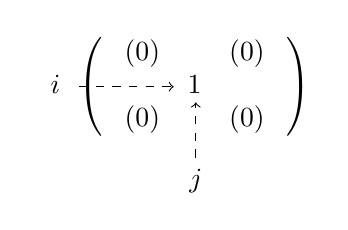
\begin{tikzpicture}
\node{$\begin{array}{c}
    \text{} \\ i \\ \text{}
\end{array}\left(\vphantom{\begin{array}{c}
    1\\ 2\\ 3
\end{array}}\right.\begin{array}{ccc}
    (0) & & (0) \\
     & 1 & \\
     (0) &  & (0)
\end{array}\left.\vphantom{\begin{array}{c}
    1\\ 2\\ 3
\end{array}}\right)$};
\draw[dashed, ->] (-1.2, 0) -- (0, 0);
\node at (0.28, -1.2) {$j$};
\draw[dashed, ->] (0.28, -0.9) -- (0.28, -0.2);
\end{tikzpicture}
\end{center}



\newpage


\subsection{Anneau des matrices diagonales}

\begin{theorem}{Anneau $\bcD_n(\bdK)$}{}
    \[ \hg{(\bcD_n(\bdK), +, \times) \ \text{est un} \ \bf{sous-anneau commutatif}.}\]
\end{theorem}

\end{document}